\section{Benchmark}
\label{sec:benchmark}

In this section we will present some experiment numbers on a simulated data-set as well as production numbers on two user facing features viz. `People You May Know' (also called PYMK) and `Viewers of this profile also viewed' (also called Browsemaps). We use two metrics to evaluate our system - faster build time and good serving latency. All tests were run on boxes running Linux 2.6.18 with Dual CPU (each having 8 cores running at 2.67 GHz), 24 GB RAM and 6 RAID 10 drives. For the MyISAM tests we ran MySQL Community Edition version 5.0.27. We start by describing the data-sets we used for our benchmarking. 

\begin{itemize}
	\item \emph{Fixed value size data-set} : The key is a long between 0 and a varying number. The value is a fixed 1024 bytes size random string. 
	\item \emph{PYMK data-set} : On logging into our site, our users are presented with recommendations of other users whom they might know and would connect with. This is presented as a store where they key is the logged in user's member id while the value is a list of integer recommended member ids. Figure \ref{distribution} shows the value size distribution for this store. 
	\item \emph{Browsemaps data-set} : Browsemaps runs collaborative filtering algorithm on members and shows you similar members when you visit a member's profile. The value is a list of 2 integers, a string and a flot. Similar to PYMK, Figure \ref{distribution} shows the value size distribution for Browsemaps. 
\end{itemize}

\begin{figure}
  \centering
    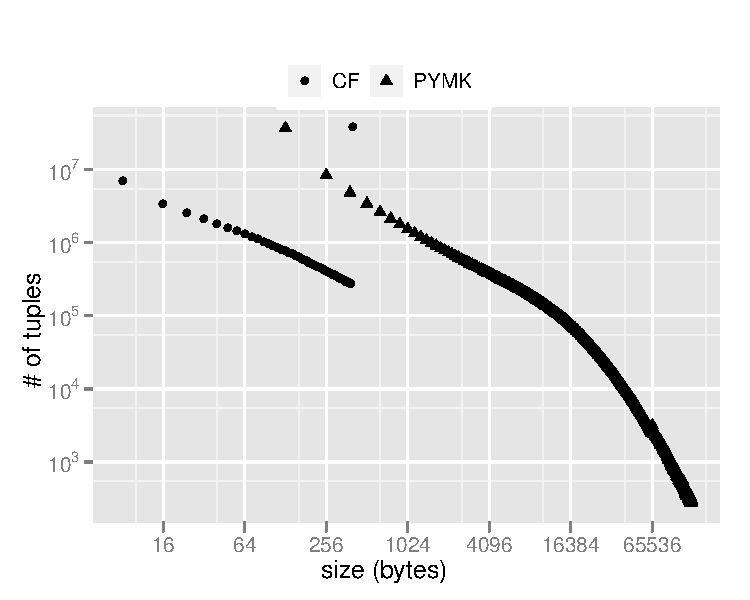
\includegraphics[scale=0.55]{images/data_distribution.pdf}
  \caption{Value size distributions for PYMK and Browsemaps. The abrupt stop is because we put a cap on the number of recommendations}
  \label{distribution}
\end{figure}

The first metric that we look into is the build times. To do a fair comparison we built all our stores for a single node. The build time in case of our Hadoop job includes the time it takes to generate the chunk mapping (map phase), shuffle the data and finally emit it to the store files (reduce phase). The number of mappers and reducer were kept fixed so as to have same amount of parallelism. This also resulted in fixed number of chunks being generated.

In case of MySQL - MyISAM test the total time only includes the completion of the \sql{LOAD DATA INFILE} command. This does not include the time it took us to extract this data, convert it into TSV format and finally copy it over to the node running MySQL single instance. Some other optimizations we did to make MySQL faster include - (a) Increasing the MySQL bulk insert buffer size and MyISAM specific sort buffer size to 256 MB each (b) Delaying the re-creation of the index to a latter time by running \sql{ALTER TABLE...DISABLE KEYS} statement before the load. 

Besides the B$^{+}$ tree structure built inside MySQL, we wanted to try to build our own B$^{+}$ tree structure tailored to Hadoop. Instead of generating chunk files in every reducer step, we generate a B$^{+}$ tree. This tree contains of a single data file (similar to the chunk data file) and a set of index files corresponding to every level of the tree. The bulk loading of the tree is done in blocks (of size $b$) i.e. we first finish the lower level's block and only then initialize a block at the next level. We then apply this rule recursively for every level as the sorted elements stream through. This bulk loading approach is efficient in that it does not require us to buffer any values in memory and can directly write to the level based index files. 

The graph in Figure \ref{build} is the build time in seconds for the above three scenarios as we increased the size of the input data-set. The block size $b$ for the B$^{+}$ was set to 340. We chose this value since our keys were 12 bytes (8 byte MD5 and 4 byte offset) long and the page size was 4096 bytes. This meant the best block size would be approximately 4096/12 $\sim$ 340. As is clearly evident MySQL takes a really long time even after being alloted a huge buffer size. The optimized B$^{+}$ on the other hand performs very well initially for small sizes but starts to deviate for larger sizes due to the extra I/O that it needs to do. In particular it needs to do extra disk writes equal to the data in the higher levels of the tree. For a fixed block size, the extra disk writes is linear with the number of tuples. The big disadvantage of the B$^{+}$ tree approach is that the serving latency is very sensitive to the block size $b$. Unfortunately setting the right value of $b$ is machine specific and hence error prone. 

\begin{figure}
  \centering
    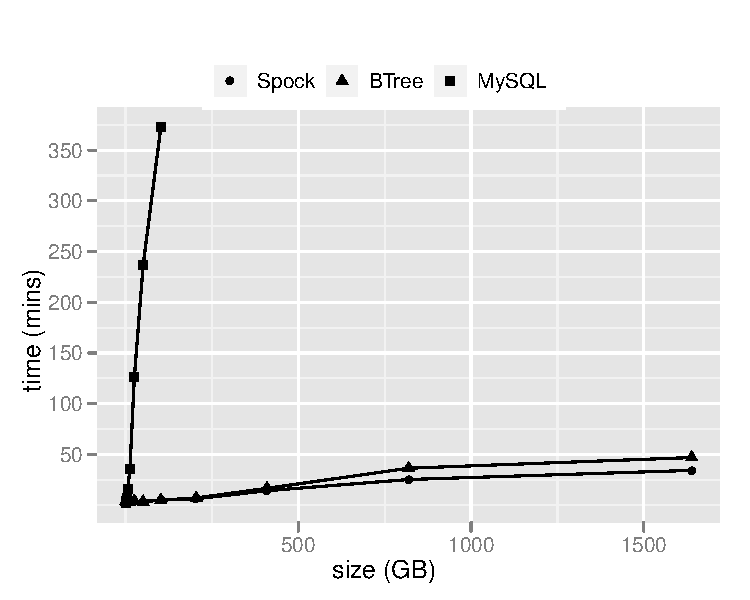
\includegraphics[scale=0.55]{images/build.pdf}
  \caption{Build time vs varying data size}
  \label{build}
\end{figure}

The next metric we benchmark is the search latency. For the random data-set we used 10 million requests with simulated values following an uniform distribution. For the PYMK and Browsemaps data-set we took a snapshot of member activity from our live Kafka stream on one of the high traffic days and used that data to generate performance numbers.

We first try to understand the performance implications of binary search vs interpolation search. In particular we were interested in measuring how fast the index can get paged into the operating system's page cache and whether the search algorithm can help with that. We ran tests on a 100GB of data on a single node with the page cache being flushed between test runs. The graph in Figure \ref{search} plots the median latency vs time. As is evident from the graph even though binary search initially starts with a very high median latency the slope of the line is steeper compared to that of interpolation search. This is because we found binary search algorithm did an average of 17.5 lookups thereby touching way more parts of the index from the very beginning. Compared to that interpolation search does only 4 lookups which hence results in an initial low search latency but comes at the expense that most parts of all the indexes are un-cached for a longer time. Our production systems are currently running on binary search due to faster cache warming process.  

\begin{figure}
  \centering
    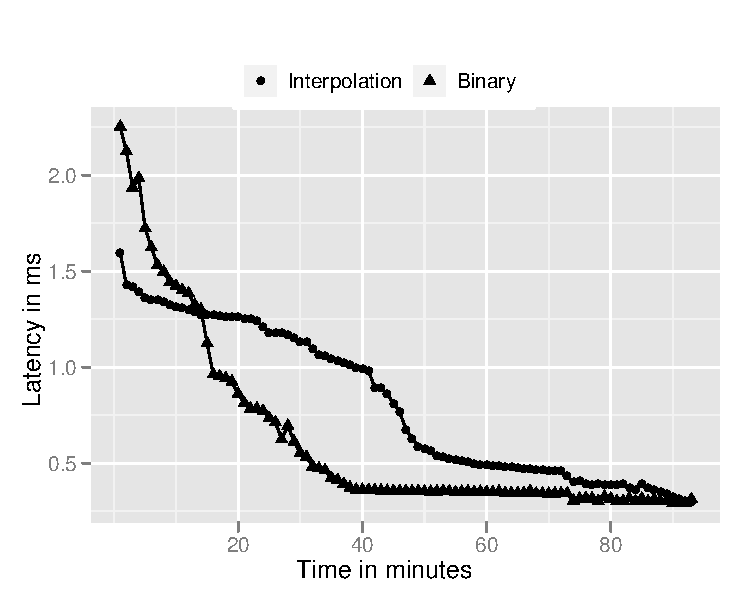
\includegraphics[scale=0.55]{images/search_1node.pdf}
  \caption{Search Latency vs Time since swap}
  \label{search}
\end{figure}

We ran the same 100 GB data-set through MySQL to get its performance numbers. Following table summaries the performance difference for a fixed throughput of 1000 queries per second. 

\begin{center}
    \begin{tabular}{ | c | c | c |  }
    \hline
     & MySQL & \projectname{} \\ \hline
    Median &   0.12 ms &  0.028	ms \\
	99th Percentile	& 45 ms & 36 ms \\
\hline
    \end{tabular}
\end{center}

To test whether the system scales well with the number of boxes, we present the latency numbers for the same random data-set but spread over 16 boxes. The data was fetched by \projectname{} at a steady rate bound by the disk or network. In our scenario we saturated the 1 Gbit line between HDFS and \projectname{} nodes. We ran the tests for both uniform as well as zipfian distribution (generation of which is further described in \cite{gray}). In particular we make sure that the `hot' elements are queried together since that simulates the general site visiting patterns of some users frequently coming to our site and generating a lot of activity. Figure \ref{16search} shows the max of the median latency of individual nodes versus different data-sizes. The `hotness' of some keys makes it very cacheable thereby giving an overall lower latency compared to the uniform distribution. 

\begin{figure}
  \centering
    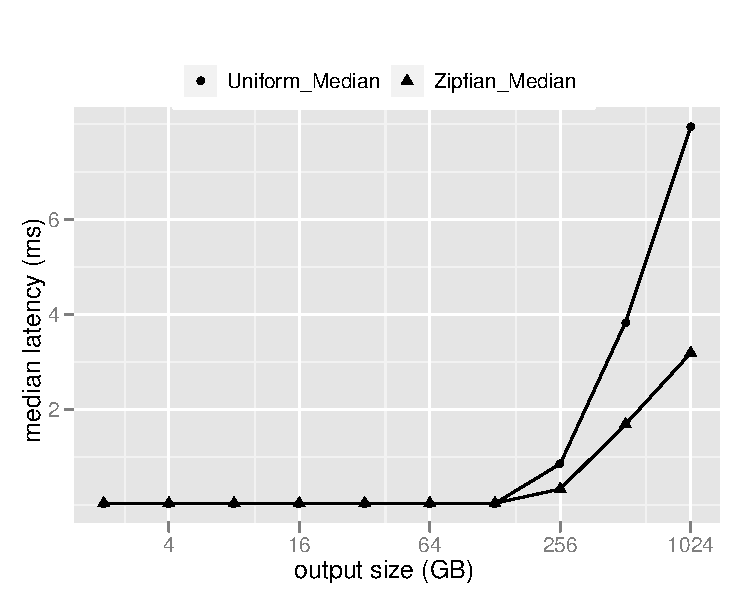
\includegraphics[scale=0.55]{images/search_16node.pdf}
  \caption{Median search latency vs varying data size for 16 node cluster}
  \label{16search}
\end{figure}


We finally present the latency numbers for PYMK and Browsemaps on our production cluster in Figure \ref{production}. This shows the average latency on the server side across all nodes immediately after a new data swap. Browsemaps has a high latency primarily because of the data size being larger than that of PYMK.

\begin{figure*}
  \centering
    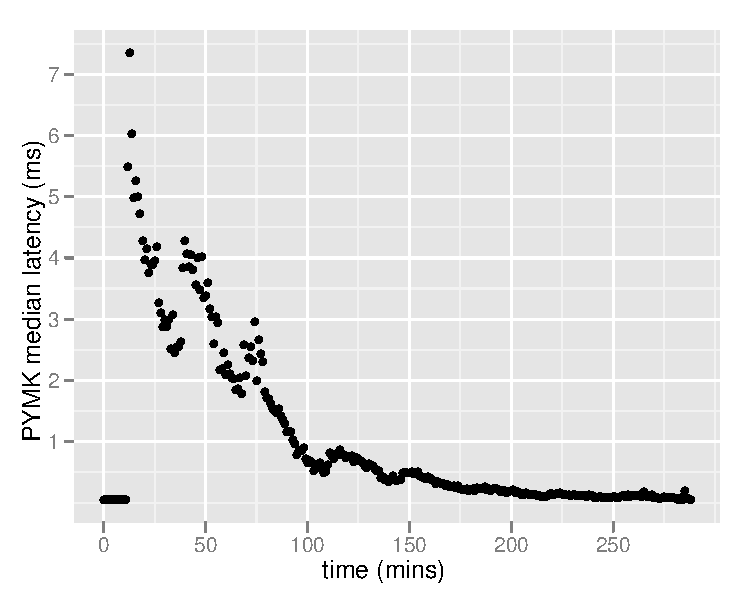
\includegraphics[scale=0.55]{images/pymk_search.pdf}
    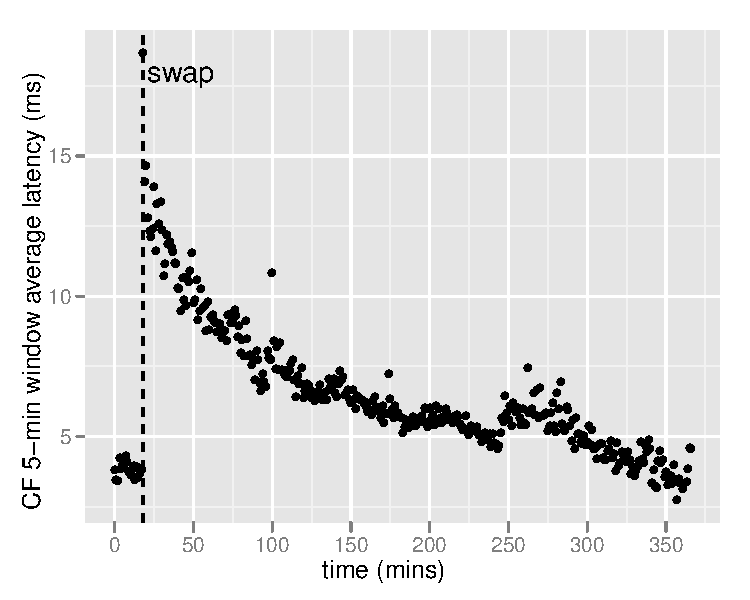
\includegraphics[scale=0.55]{images/browsemap_search.pdf}
  \caption{Latency vs Time for PYMK and Browsemaps}
  \label{production}
\end{figure*}

